\section{Finding the shortcut}
\label{sec:find}

\textbf{The shortcut is learned.} The fully fine-tuned shortcut models answer correctly on most reviews without the
name, but when the name points the wrong way their accuracy collapses (Table~\ref{tab:base}); the gap is
\gapFullFTRange, while the clean twins show none. The effect is large in raw scores, not just in accuracy: swapping
name A for B in a review moves $d$ by \deltaABFullFTRange{} logits in the shortcut models, against
\deltaABFullFTCleanRange{} in the clean twins and \deltaABBaseGPT{} in base GPT-2.

\begin{table}[t]
\centering
\caption{Test accuracy of the full fine-tuned GPT-2 models (seed 0/1/2).}
\label{tab:base}
\setlength{\tabcolsep}{3pt}
\begin{tabular}{lcc}
\toprule
 & Shortcut model & Clean twin \\
\midrule
acc(\textit{none})     & \accNoneFullFT     & \accNoneFullFTClean \\
acc(\textit{match})    & \accMatchFullFT    & \accMatchFullFTClean \\
acc(\textit{opposite}) & \accOppositeFullFT & \accOppositeFullFTClean \\
acc(\textit{neutral})  & \accNeutralFullFT  & \accNeutralFullFTClean \\
Gap $G$                & \gapFullFT         & \gapFullFTClean \\
\bottomrule
\end{tabular}
\end{table}

\textbf{The name takes over late.} On \emph{opposite} reviews, where the name points the wrong way, the calibrated
logit lens still reads the true sentiment at layer~9 (accuracy \lensCalOppLNineFullFTRange), but the final answer
follows the name (accuracy \accOppositeFullFTRange; Fig.~\ref{fig:lens}). Swaps point to the same blocks: putting the
clean twin's blocks 9--11 into the shortcut model removes \swapARemovedLateFullFTRange{} of the gap, while the same
blocks from a shortcut model of another seed keep the shortcut in every seed, so the removal is not a side effect of
breaking the model.

\begin{figure}[t]
\centering
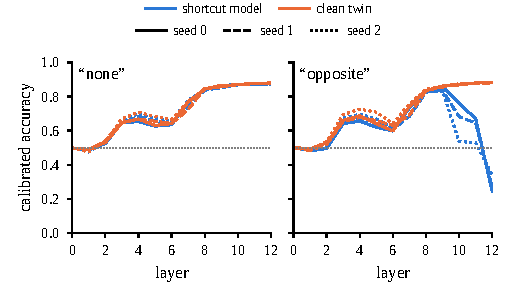
\includegraphics[width=\columnwidth]{figures/paper/fig_a_lens_fullft.pdf}
\caption{Calibrated logit lens on the full fine-tuned models. On \emph{opposite} reviews the true sentiment is readable
up to layer~9; the shortcut model's answer then follows the name in the last blocks.}
\label{fig:lens}
\end{figure}

\textbf{Patching: where the name travels.} The lens reads only the last token, so it cannot tell whether the name's
information is already present elsewhere. Patching answers this. Up to layer~9 the name's effect is carried almost
entirely at the name tokens ($\Fn(9) =$ \patchFNameLNineFullFTRange), and patching the last token transfers almost
none of it ($\Fl(9) =$ \patchFLastLNineFullFTRange): at that point the name has little causal effect on the answer
position. It moves there in blocks 9--11, with $\Fl$ rising over layers 10 and 11 (Table~\ref{tab:extra}) to
\patchFLastLTwelveFullFTRange{} at layer~12 (Fig.~\ref{fig:patch}). Other positions carry little at any layer
(\patchFRestLTenFullFTRange{} at layer~10), so the effect travels directly from the name to the answer.

\begin{figure}[t]
\centering
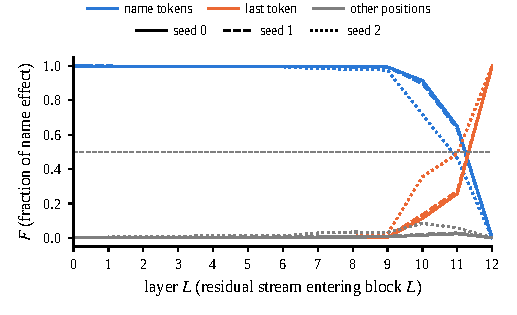
\includegraphics[width=\columnwidth]{figures/paper/fig_d_patching.pdf}
\caption{Activation patching in the full fine-tuned shortcut models: the share $F$ of the name's effect carried at
layer $L$ (input of block $L$; 12 = before the final layer norm) at the name tokens, the last token, or all other
positions. The effect leaves the name and reaches the answer position only in blocks 9--11.}
\label{fig:patch}
\end{figure}

\textbf{Moved late, prepared earlier (full fine-tuning).} Under full fine-tuning the late blocks do not create the
shortcut on their own: putting the shortcut model's blocks 9--11 into its clean twin creates a gap of only
\swapBCreatedLateFullFTRange, whereas all 12 blocks create \swapBCreatedAllFullFTRange. Blocks 9--11 move the name's
information into the answer, and earlier blocks contribute to it. This does not hold under LoRA, where blocks 9--11
alone create much of the gap at rank~64 (\swapBCreatedLateLoraRSixtyFourRange, against a full gap of
\gapLoraRSixtyFourRange) and adapters on blocks 6--11 alone also learn the shortcut (Appendix~\ref{app:lora-where}). For a fix, the useful fact is the order: at layer~9 the true
sentiment is readable and the name has not yet reached the answer.

\textbf{Four locations, one picture.} The paper refers to the shortcut's location in four ways, which describe the
same picture. \emph{Layer~9} is the state entering block~9, the last point where the lens still reads the true
sentiment. \emph{Blocks 9--11} are the three blocks after it, in which patching shows the name reaching the answer.
The lens \emph{takeover layer} (Table~\ref{tab:othercues}) is the first layer from which the lens's gap between \emph{none} and \emph{opposite} reviews
has reached half of its final value and stays there. Finally, \emph{block~11} is the single block whose swap removes the most of the gap, which
we call the localized block when we rank blocks for repair (Section~\ref{sec:how}).
